
\section{Introduction}

% In formal system analysis, abstraction is a double-edged sword. On one
% hand, abstracting away irrelevant details and focusing on the most
% critical aspects of a system keeps the analysis tractable. On the
% other hand, some of the omitted details may actually be 

In a typical analysis process, the analyst constructs a model that
describes the system and its environment, and applies an analysis
technique, such as model checking and theorem proving, to determine
whether the model satisfies a given property. If the analysis
completes without finding a violation, the analyst may be inclined to
assume that the actual system satisfies the desired property. 

In practice, the system might suffer from a failure, despite
the successful analysis, because the model used in the analysis
(purposely or inadvertently) omits details about the system that could
lead to a violation of the property. The analyst, for instance, may
decide to leave out the description of a seemingly unimportant system
function, or simply be unaware of certain classes of interactions with
the enviroment. For example, an ATM system for a major bank in UK,
which relied on a provably correct cryptographic mechanism to protect
a PIN number on a card, suffered from security failures because the
designer had neglected to consider the possibility that a malicious
person could simply modify the account number on his card to that
of another customer (which enabled him to withdraw money from the victim's
account)~\cite{anderson-needham}.

Constructing a model that is sufficiently detailed to account for
possible failures, however, is a challenging task that requires
significant expertise in the problem domain. The analyst---often the
designer of the system---may initially have a rather limited, partial
knowledge about the system, or ignore details that appear irrelevant
to its core functionality. As the analyst improves her understanding
of the system, its operating environment, and potential failures, she
may incrementally elaborate the existing system model and perform
multiple iterations of analysis, each time discovering new violations
that the prior analyses had ruled out. Unfortunately, this process is
often carried out in an ad hoc, manual fashion.

\begin{figure}[!t]
\centering
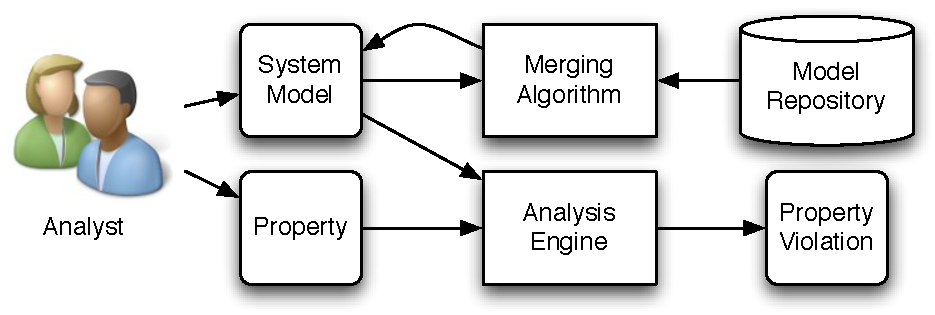
\includegraphics[width=0.60\textwidth]{diagrams/overview}
\caption{Overview of our framework on model construction and analysis.}
\label{fig-overview}
\end{figure}

In this paper, we propose a framework to aid the analyst in
incremental construction and analysis of a system model. Our framework
consists of three key components, as shown in
Figure~\ref{fig-overview}: (1) a repository of models that encode
partial knowledge about the problem domain, (2) an algorithm that
merges two independent models of a system, and (3) an analysis engine
that checks whether a system model satisfies a given property, and if
not, produces a counterexample. In a typical workflow, the analyst
begins by constructing a partial model of the system, and runs an
initial analysis to check the system against a desired property. The
analyst then incrementally elaborates the initial model into a more
detailed one by merging it with the existing models in the repository,
one-by-one. After every merge step, the analyst re-runs the
analysis on the elaborated model to detect any potential violations
that were absent from prior analyses.

A technical challenge in composing two independent models is that they
may not be amenable to composition due to \textit{abstraction
  mistmach}. The two models may describe some aspect of the system at
different layers of abstraction, using different sets of vocabulary
terms, so standard composition techniques that connect components at
their interfaces may fail. To resolve this mismatch, we allow the
analyst to specify relationships between various parts of the two
models. Our merging algorithm then automatically constructs a new
model that is the result of composing two mismatched models according
to the specified relationships.

Our goal is not to completely automate the model construction process;
we still rely on the analyst to use insights about the system to drive
the model elaboration process, and interpret the output of the
analysis engine to devise meaningful fixes to the model. Our framework
facilitates the model construction and analysis process in the
following ways:
\begin{itemize}
\item \textbf{Knowledge reuse}: A repository of generic domain models,
  constructed by a domain expert, can be reused for analysis of
  multiple systems. For example, a repository of models about common
  attacks on web applications may be used to analyze the security of
  multiple, independent web protocols.
\item \textbf{Incrementality}: Instead of having to come up with a
  complete, monolithic model of a system, the analyst can
  incrementally explore different aspects of the system, one at a
  time. For example, the analyst may rank the available attack models
  in the order of their criticality, and analyze the system for the
  most pressing issues first.
\item \textbf{Adaptiveness}: As the repository is updated with new
  models (e.g., newly discovered attacks or new operating environments),
  the analyst may repeat the analysis process without having to build
  the model from the scratch.
\end{itemize}

\textbf{Contributions} The contributions of this paper are as
follows:
\begin{itemize}
\item A framework for incremental construction and analysis of a
  system model that leverages a domain-specific model repository,
\item A technique for merging two potentially mismatched models,
\item An implementation of the framework, including a language for
  specifying system models and an automated analysis engine built on
  top of a model finder, and
\item Application of the framework to the analysis of two well-known
  web protocols, OAuth~\cite{oauth} and OpenID~\cite{openid}.
\end{itemize}

\textbf{Outline} This paper is structured as
follows. Section~\ref{sec-overview} provides an overview of our
framework with an example from an online news paywall system.
Section~\ref{sec-formalism} introduces the underlying formalism for
modeling systems. Section~\ref{sec-merging} describes the types of
relationships that the analyst can specify between two potentially
mismatched models, and the merging algorithm that composes the two
based on the given relationships. Section~\ref{sec-implementation}
discusses the implementation of the modeling formalism as a
domain-specific language as well as an automated analysis of merged
models. Section~\ref{sec-case-study} describes the case studies on
applying our approach to the OAuth and OpenID protocols. The paper
concludes by discussing the related work
(Section~\ref{sec-related-work}), and the potential benefits and
limitations of our approach (Section~\ref{sec-discussion}).

% However, there are a number of risks in reaching such a conclusion:
% (1) the analysis technique used may be unsound or incomplete, (2) the
% analyst may have specified an incorrect property, or (3) the model
% used in the analysis may (purposely or inadvertently) omit details
% about the system that, in reality, could lead to a violation of the
% property.
